\section{The full source, its endpoint, and the ideal recovered from all
covers}\label{the-full-source-its-endpoint-and-the-ideal-recovered-from-all-covers}

This continuation retains the preceding original-zeta calculations and
adds their full source-to-Hardy comparisons. The entire proofs and
mathematical reviews follow. The support notation and its retractions
remain unchanged; all coefficient operations occur after the complete
arithmetic reconstruction.

GDE calculates the two ordered Gaussian energies, original divisor and
Hilbert traces, determinants, degree action and parameter comparisons.
GSP/GSI supply the original source's complete spectral synthesis.
NHR/NAD receive Noor's original coefficients and prove the Hilbert
comparisons; NHD/NHDA construct the complete dual graph. NHJ then proves
that the corrected integer tests inject the entire original strong dual
into disk-holomorphic functions. ABH/AHR apply this to the actual
reflected specialization boundary, with a trace-class receiver, the full
Gram matrix, exact raw-cover projection defect and all-scale
reconstruction in trace norm. Each of these maps retains its own domain
and kernel.

\begin{figure}
\centering
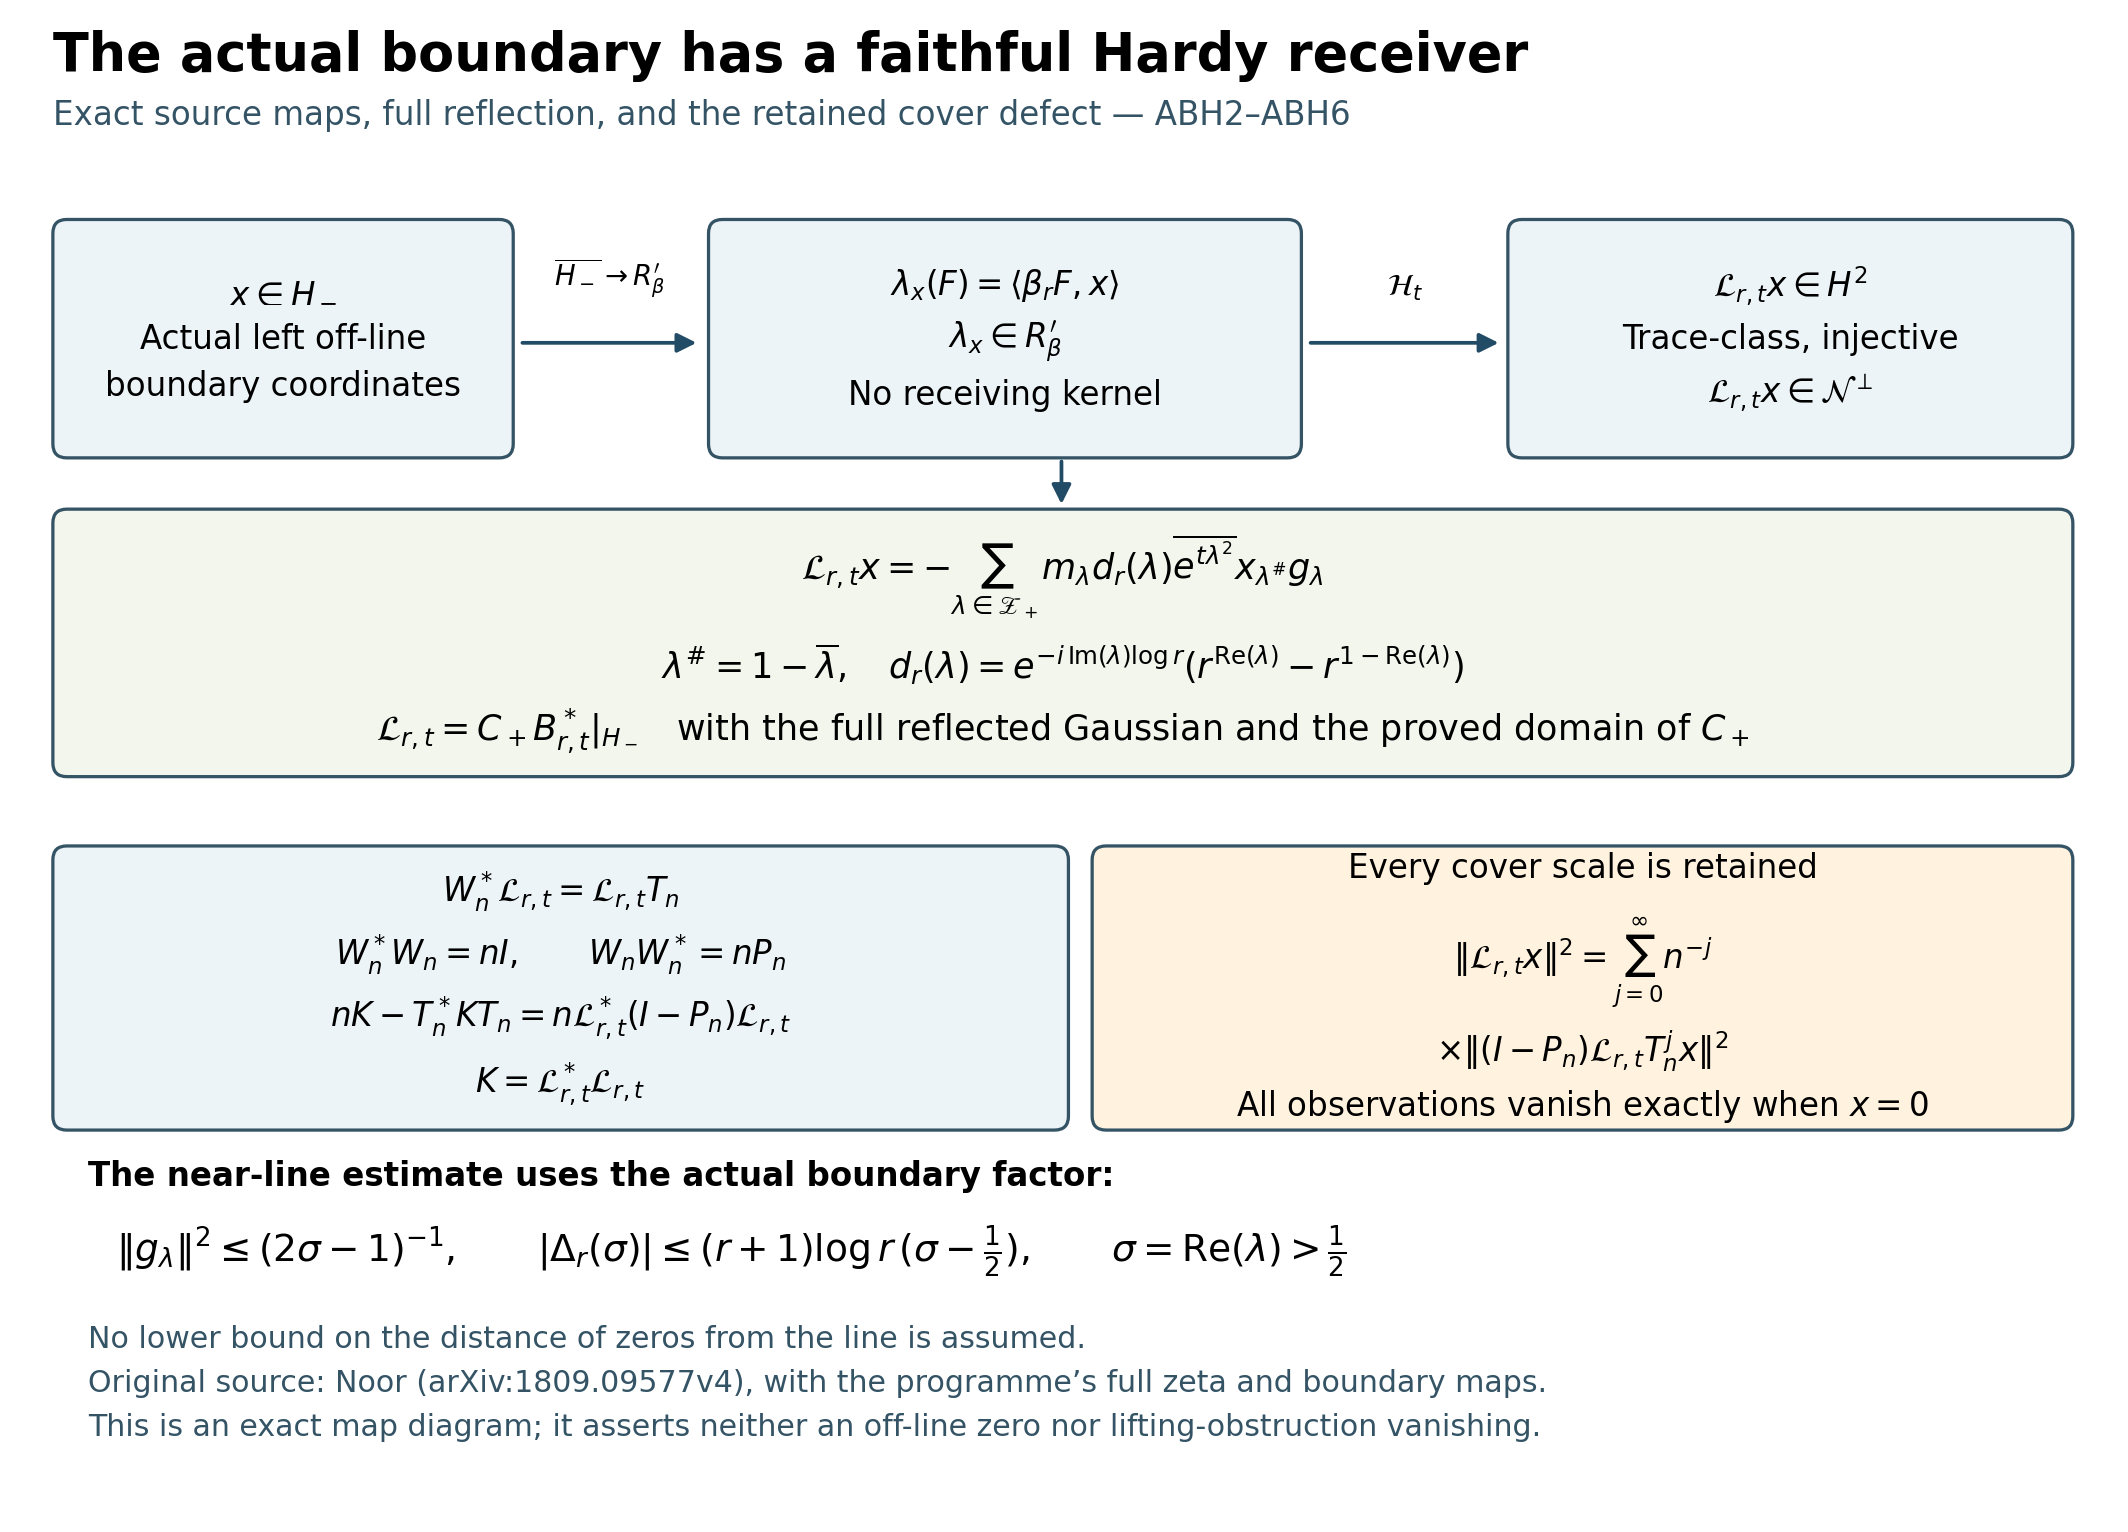
\includegraphics[width=1\linewidth,height=\textheight,keepaspectratio,alt={The actual reflected boundary maps through the full specialization dual into Noor's Hardy space. ABH2--4 prove injectivity, absolute convergence and the exact GDE factorization. ABH5--6 and AHR6--7 retain the raw degree and show that observations at every scale reconstruct the full norm and vector. The near-line estimate includes its exact constant and needs no positive lower bound on a zero's displacement. This is an exact map diagram, not a numerical sample. The original Hardy construction is S. Waleed Noor, arXiv:1809.09577v4.}]{actual_hardy_boundary.png}
\caption{The actual reflected boundary maps through the full
specialization dual into Noor's Hardy space. ABH2--4 prove injectivity,
absolute convergence and the exact GDE factorization. ABH5--6 and
AHR6--7 retain the raw degree and show that observations at every scale
reconstruct the full norm and vector. The near-line estimate includes
its exact constant and needs no positive lower bound on a zero's
displacement. This is an exact map diagram, not a numerical sample. The
original Hardy construction is S. Waleed Noor, arXiv:1809.09577v4.}
\end{figure}

The new source-level result NCI proves that the complete family of cover
discrepancies generates exactly the original nontrivial-zero ideal,
including every zero multiplicity, after closure in the original strip
topology. It also proves that the algebraic principal image is strictly
smaller than that ideal. The original full-jet quotient is therefore
recovered from the complete discrepancy, with the exact quotient
topology. All-cover covariance and stability in the original
Hardy-domain slice characterize its continuous dual.

NPE retains the actual pole of the correction as a meromorphic source
extension. Its residue character, nonzero endpoint extension,
two-dimensional square-zero action, split full-ideal pushout and unique
section are calculated. The full extended analytic receiver is injective
and exactly covariant before quotienting. Its Hardy graph includes the
retained endpoint coordinate. The independent endpoint review proves the
exact comparison by multiplication by s, including the changed embedded
subspace and both distinct pushouts. These maps prevent a change of
presentation from silently deleting an endpoint.

\begin{figure}
\centering
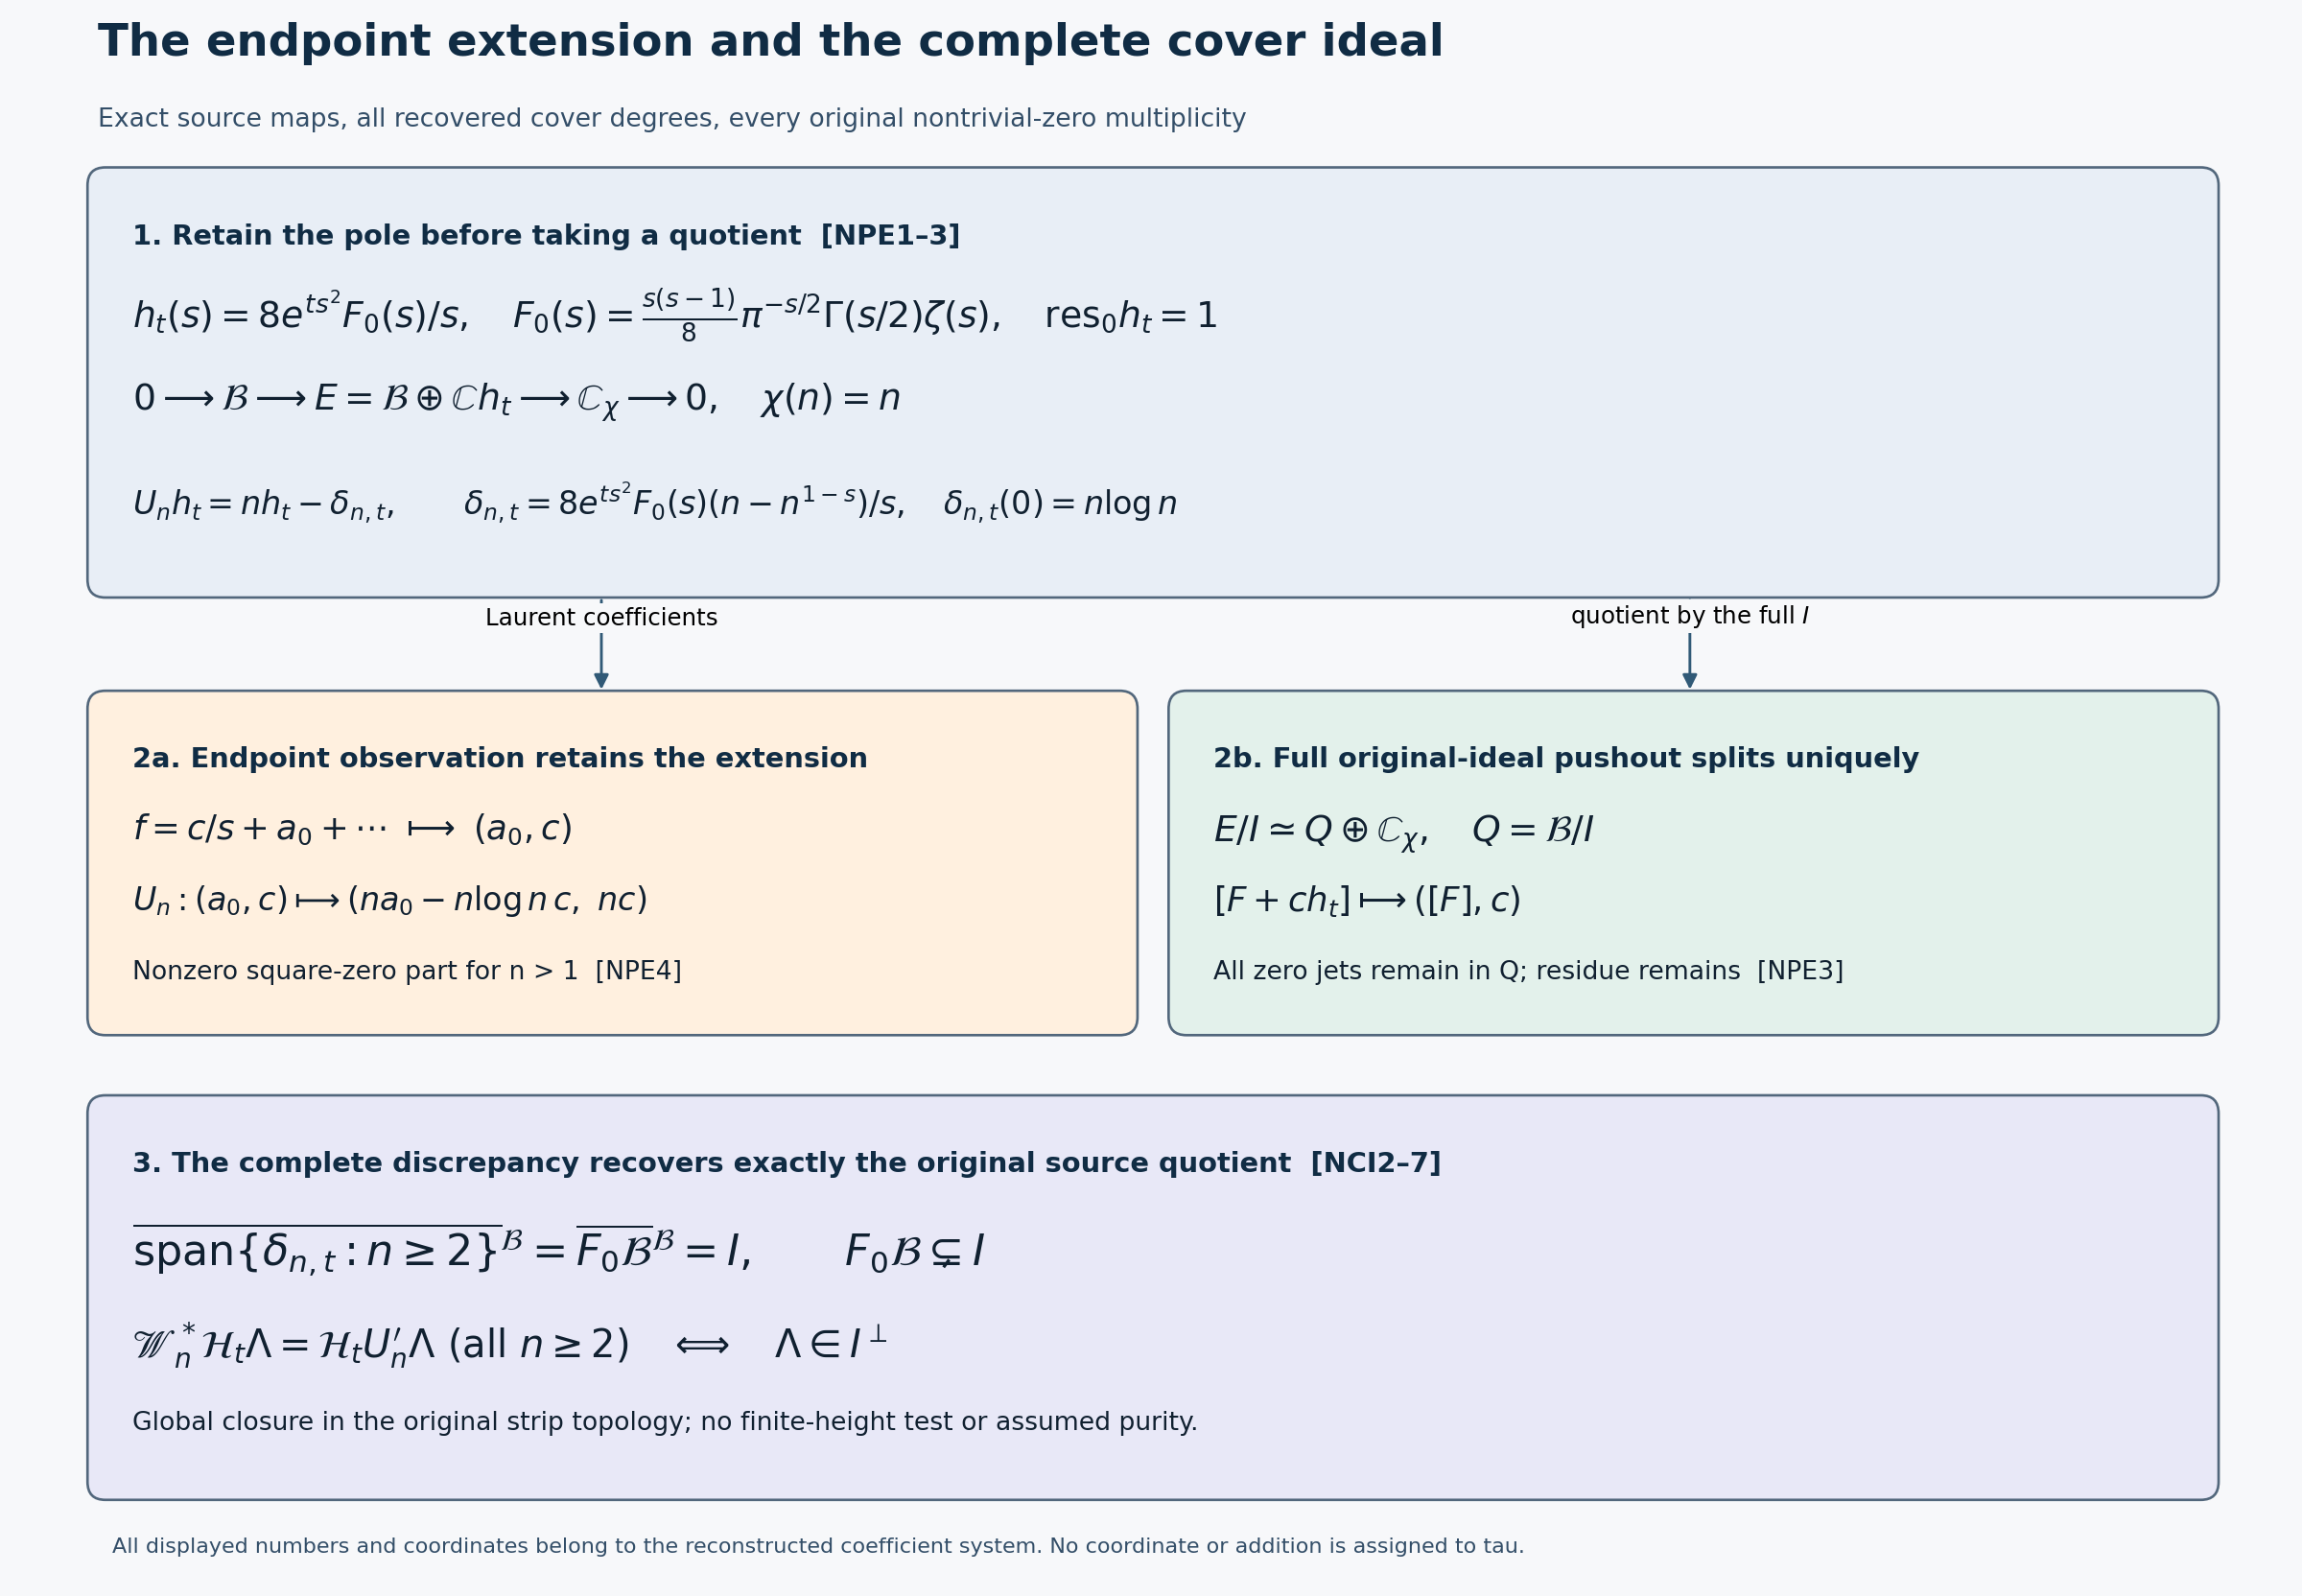
\includegraphics[width=1\linewidth,height=\textheight,keepaspectratio,alt={NPE1--4 calculate the original residue-one extension, its exact cover cocycle, and two different observations: the Laurent-coefficient receiver retains a nonzero square-zero component, while the full original-ideal pushout splits uniquely. The displayed direct sum for E is a vector-space presentation; the cover action mixes its terms. NCI2--7 prove the closed-span identity and the resulting exact covariance characterization on the original entire-source dual. Every zero jet remains in Q and the residue remains in the additional line. The larger pole-inclusive graph is distinguished explicitly in NPE7--8. This is a diagram of proved maps and formulas, not a plot or an RH assumption. Human source for the coefficient receiver: S. Waleed Noor, arXiv:1809.09577v4.}]{endpoint_cover_ideal.png}
\caption{NPE1--4 calculate the original residue-one extension, its exact
cover cocycle, and two different observations: the Laurent-coefficient
receiver retains a nonzero square-zero component, while the full
original-ideal pushout splits uniquely. The displayed direct sum for E
is a vector-space presentation; the cover action mixes its terms.
NCI2--7 prove the closed-span identity and the resulting exact
covariance characterization on the original entire-source dual. Every
zero jet remains in Q and the residue remains in the additional line.
The larger pole-inclusive graph is distinguished explicitly in NPE7--8.
This is a diagram of proved maps and formulas, not a plot or an RH
assumption. Human source for the coefficient receiver: S. Waleed Noor,
arXiv:1809.09577v4.}
\end{figure}

The endpoint comparison preserves the original zeta pairing. In the open
right half of the critical strip, its evaluation receiver is orthogonal
to Noor's original tests exactly at the original zeta zeros. Exact cover
covariance on the enlarged source is a different proved property, and
its full remaining degree defect is retained. None of these calculations
asserts the original geometric weight-separated lifting vanishing or a
resolution of RH.

NJS and SSR then test the residue section itself in this unchanged
source. The original zeta section and the Gaussian section are related
by an explicit continuous shear, but their zero-coordinate observations
select different invariant subspaces. The full original divisor survives
as a graph in the new coordinates. RSS extends this calculation to every
polynomial section with residue one: its discrepancy span is exactly the
corresponding full finite-jet ideal. This identifies the mathematical
data supplied by the observation choice while retaining the original
source, ideal and receiver.

\begin{figure}
\centering
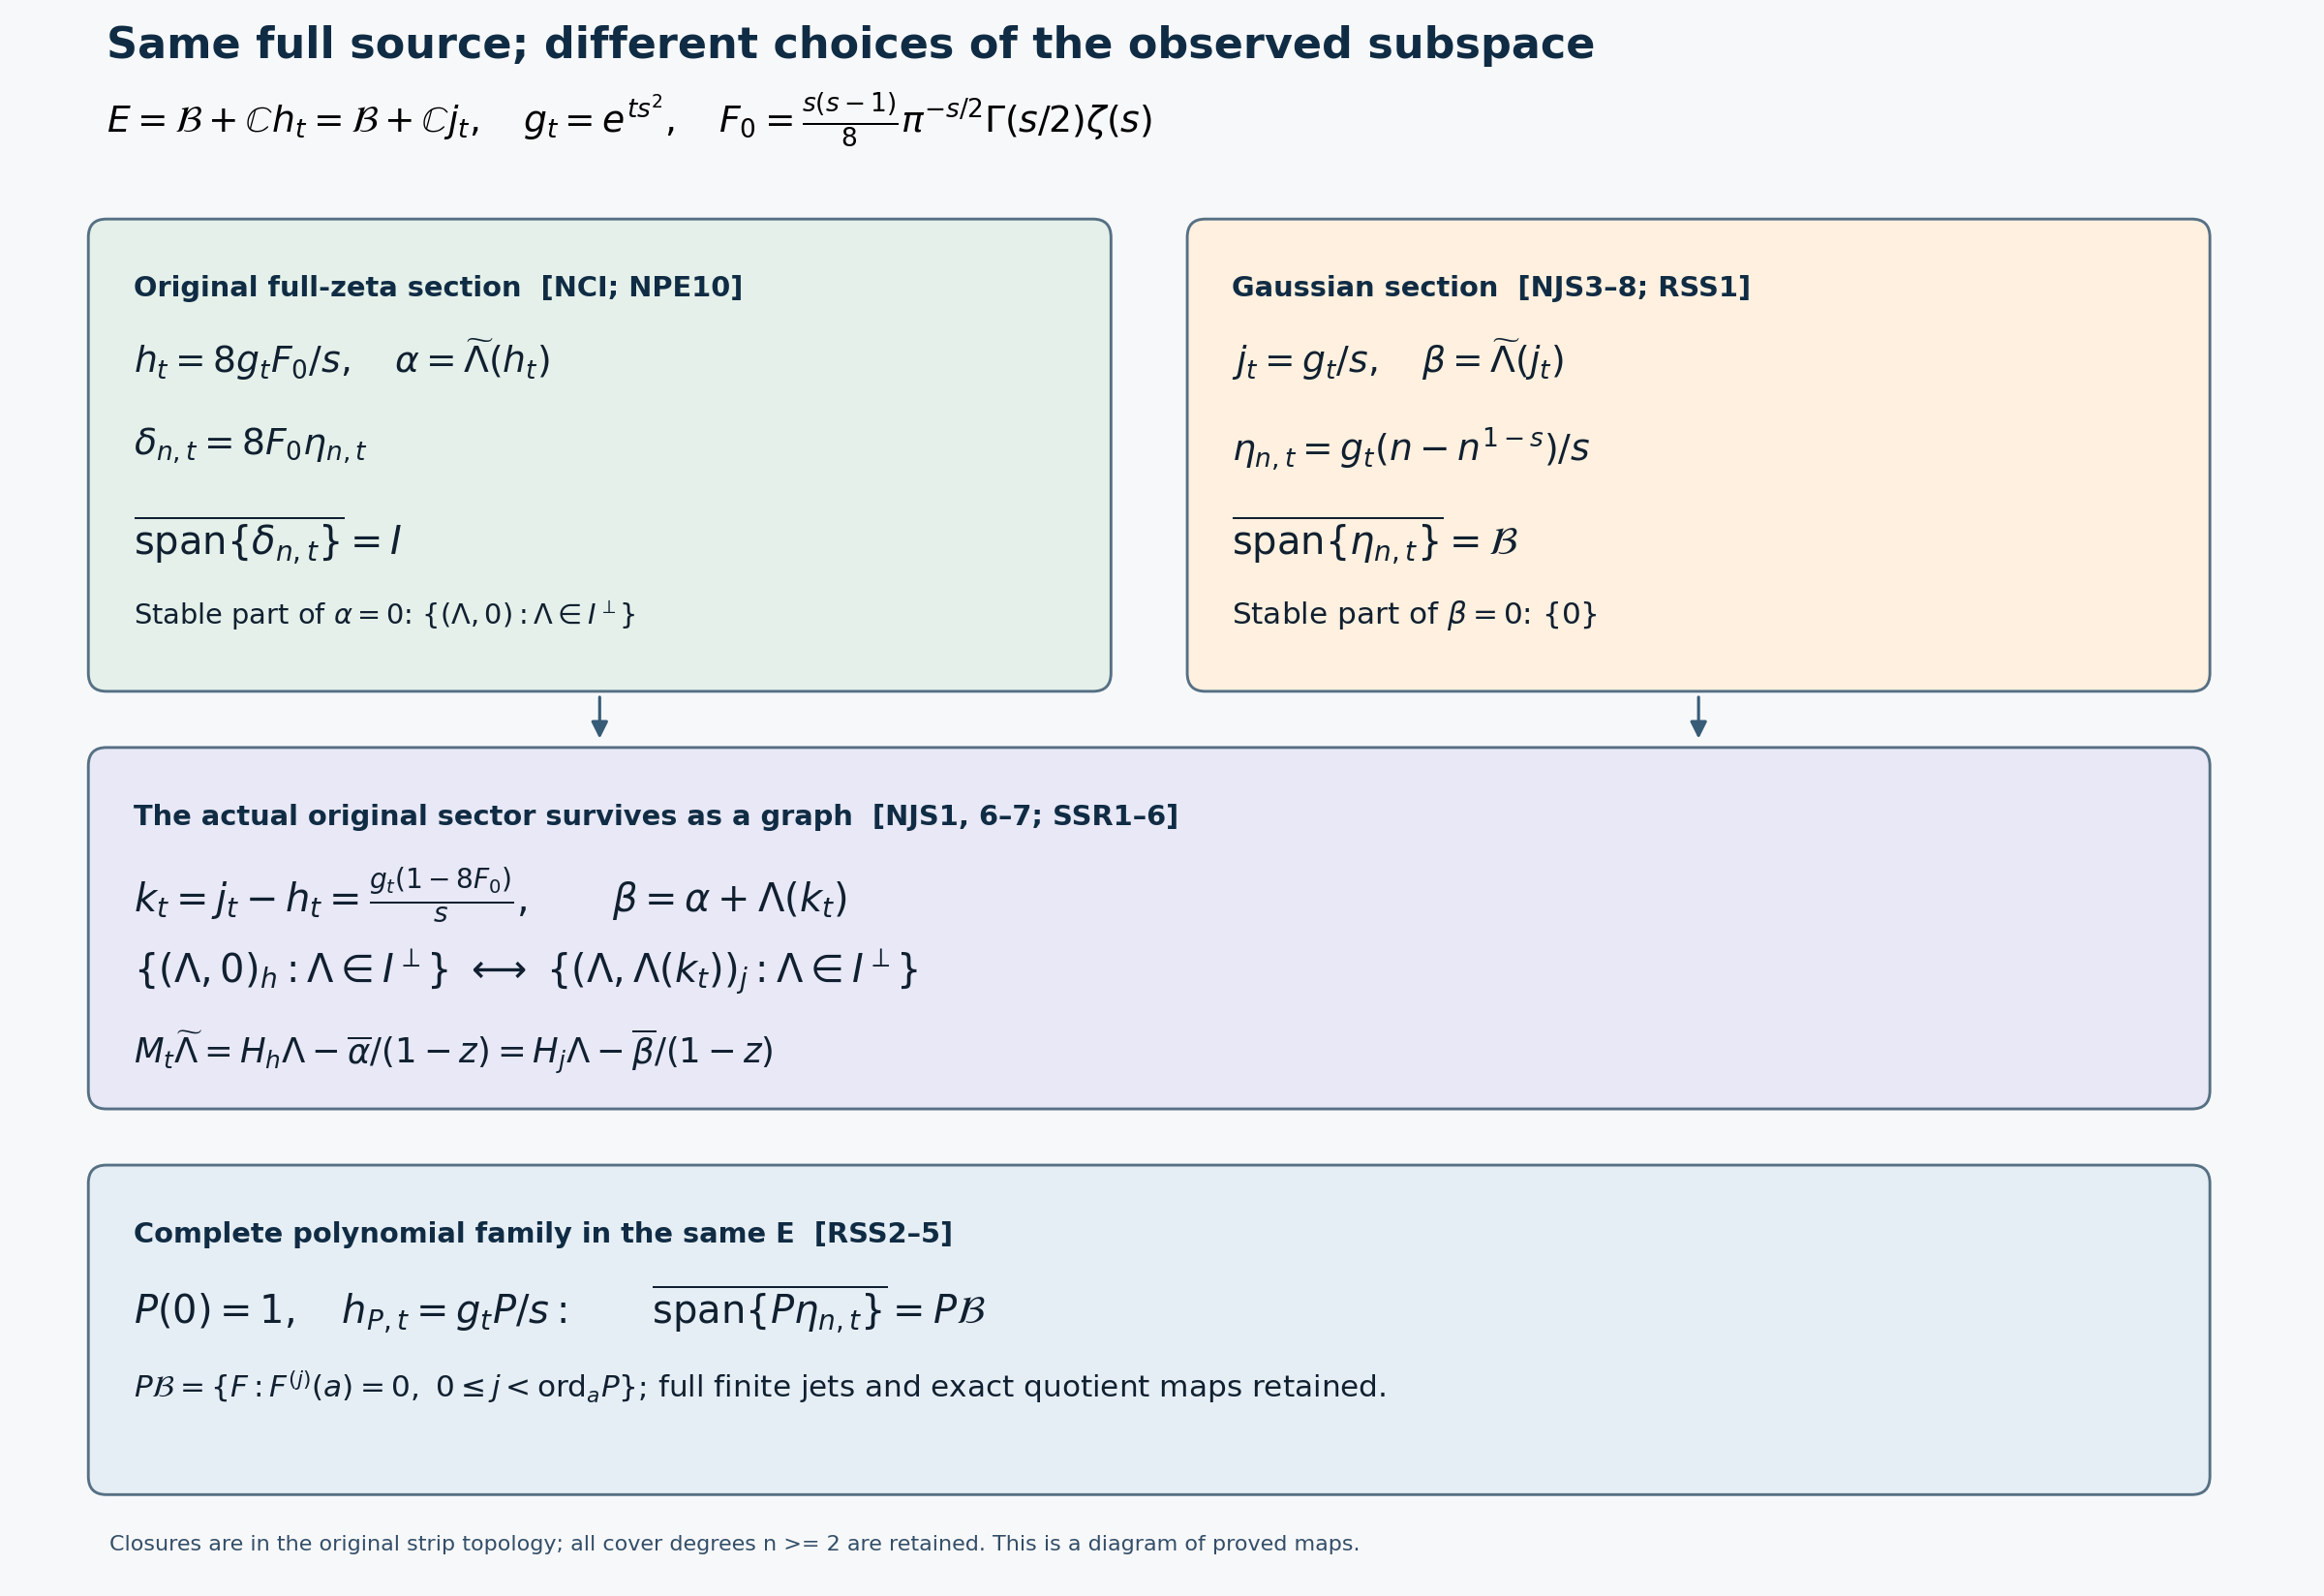
\includegraphics[width=1\linewidth,height=\textheight,keepaspectratio,alt={The same meromorphic source and cover action admit different residue sections. NJS1--8 and SSR1--6 prove the exact primal and dual shears, the two discrepancy spans, and the invariant graph that preserves the original zeta sector. RSS1--5 prove the complete polynomial family and its exact maps to the original full-jet quotient. All closures use the original strip topology. The source multiplier retains every displayed original factor; no coordinate or operation is assigned to tau. The statement concerns a chosen observed subspace, not a disappearance of the full source.}]{residue_section_comparison.png}
\caption{The same meromorphic source and cover action admit different
residue sections. NJS1--8 and SSR1--6 prove the exact primal and dual
shears, the two discrepancy spans, and the invariant graph that
preserves the original zeta sector. RSS1--5 prove the complete
polynomial family and its exact maps to the original full-jet quotient.
All closures use the original strip topology. The source multiplier
retains every displayed original factor; no coordinate or operation is
assigned to tau. The statement concerns a chosen observed subspace, not
a disappearance of the full source.}
\end{figure}

The underlying geometric programme continues to use Connes--Consani,
\href{https://arxiv.org/abs/0903.2024v3}{Schemes over F1 and zeta
functions, §5}, and Deligne,
\href{https://numdam.org/item/PMIHES_1980__52__137_0/}{Weil II §3.6}.
The new coefficient constructions do not assign a geometric weight
filtration by analogy. The author-source reading ledgers distinguish
complete programme-proof reading from the stated coverage of human
sources.

The preceding 519-page edition remains frozen. Draft-status sentences in
the retained incoming sources describe their original production stage;
the present edition's acceptance and source manifest records their
receiving review. Historical private working records, correspondence,
and cancelled programme supplements are not included in this
continuation. The original sources and receiving typography changes,
where any occur, are identified separately. New mathematics is never
attributed to the frozen earlier cutoff.
